



























%\begin{document}

	\chapter{Introducción al Aprendizaje Automático}{\label{Cap1}}	

%        https://www.oreilly.com/library/view/introduction-to-machine/9781449369880/ch01.html

        %        Introducción general a la teoría del Aprendizaje Estadístico

El Aprendizaje Automático (AA) (o Machine learning en Inglés) es la extracción del conocimiento contenido de los datos.  Este es un campo de investigación donde se interceptan las áreas de conocimiento de estadística, inteligencia artificial, y la ciencia de la computación. También se conoce como análisis predictivo o aprendizaje estadístico. La aplicación de los métodos del aprendizaje automático  se han vuelto omnipresentes   en la vida cotidiana en los últimos años, que va desde la simple recomendación de una película,  qué comida ordenar,  cuál  producto comprar,  o reconociendo a sus amigos adentro una foto, muchos sitios Web modernos y dispositivos tienen algoritmos de aprendizaje de automático  en su núcleos. Cuando inspeccionamos en un sitio Web como Facebook, Amazon, o Netflix, es muy probable encontrar  en cada parte del sitio multiples modelos de Aprendizaje Automático. \\

  %     “ ” 
  
Por otro lado, en las aplicaciones comerciales, el aprendizaje automático hoy en día ha tenido una gran influencia  en la forma en que dirigen sus investigaciones con los datos. Las herramientas introducidas en este libro han sido aplicadas a una diversidad de problemas científicos, tales  como entender el comportamiento de las estrellas, encontrando planetas distantes, descubriendo partículas nuevas, analizando secuencias de ADN, y  suministrar tratamientos personalizados contra el cáncer o cierta enfermedad.\\

 % Your application doesn’t need to be as large-scale or world-changing as these examples  in order to benefit from machine learning, though.    Sin embargo, su aplicación no necesita ser tan de gran escala o querer cambiar el mundo  como estos ejemplos para sacar provecho de aprendizaje de máquina.
 
 En este capítulo, se expone la idea general del por qué  aprendizaje automático se ha vuelto tan popular y  se  discute qué clases de problemas pueden ser solucionadas usando las técnicas del AA. Además se introducen los conceptos importantes, y se muestra  cómo puede construir su primer modelo de AA.\\

\section{¿Por qué el Aprendizaje Automático o Machine Learning? }

En los primeros días de las aplicaciones "{}automatizadas"{}, muchos sistemas utilizaban  reglas de código manual como  "{}if"{}  y  "{}else"{}  para procesar datos o para ajustar a la entrada del usuario.
Pensando en un filtro spam, cuyo trabajo es mover apropiadamente los mensajes entrantes de correo electrónico spam a una carpeta llamada spam.  Usted podría hacer una lista negra de palabras que darían como resultado un correo electrónico marcada como spam.      Éste sería un ejemplo del uso un sistema experto de regla para diseñar una aplicación "{}automatizada"{} o inteligente.   Elaborando   manualmente las reglas de decisión son  factibles  algunas aplicaciones, en particular en aquellos casos en que se  tiene todo un conocimiento completo  del proceso a modelar. Sin embargo, el uso de  reglas de código manual para la toma decisiones tienen dos desventajas principales:
 
 %  Piense acerca de un filtro del correo electrónico
\begin{itemize}
	
	\item La lógica requerida para tomar una decisión es específica para un sólo dominio y una tarea. Cambiar la tarea aun  ligeramente podría requerir reescribirla  para todo el nuevo sistema (una nueva versión).

   \item   Diseñar las  reglas requiere un profundo conocimiento de cómo debería ser una decisión hecha por un experto humano.

\end{itemize}


  Un ejemplo que está de moda y dónde el código manual falla es el problema de detectar caras adentro una  fotografías  (imágenes).   Hoy en día, cada teléfono inteligente puede detectar una cara en una imagen. Sin embargo, la detección de una cara en imágenes  fue un problema sin resolver hasta  el 2001. 
   
 El problema principal es que la forma en que la imágenes en pixeles son “percibidos” por la computadora es muy diferente de cómo perciben los humanos una cara. Esta diferencia en representación hace básicamente  imposible para un humano obtener un buen conjunto de reglas para describir lo que constituye una cara en una imagen digital.\\
 
  
 Sin embargo, usando las técnicas del aprendizaje automático aplicadas a una gran colección de imágenes de caras, es suficiente para que un algoritmo determine qué características se necesita para identificar una cara.
 


\subsection{Problemas que puede resolver el Aprendizaje Automático}


%   most successful =  más exitosos 

Los tipos de algoritmos de aprendizaje automático más exitosos son aquellos que automatizan  procesos de toma de decisiones generalizando a partir de ejemplos conocidos. Esta configuración,  se conoce como aprendizaje supervisado, el usuario proporciona al algoritmo pares de  entradas y salidas deseadas, y el algoritmo encuentra una manera de producir la salida deseada dada una entrada.

En particular, el algoritmo puede crear una salida para una entrada nunca antes vista sin la ayuda de un humano. Volviendo a nuestro ejemplo  de clasificación de spam, utilizando el aprendizaje automático, el usuario proporciona al algoritmo una  gran cantidad de correos electrónicos (que son la entrada), junto con información sobre  si algunos  de estos correos electrónicos son  spam (que es el resultado deseado). Dado un nuevo  correo electrónico, el algoritmo producirá una predicción sobre si el nuevo correo electrónico es  correo no deseado. Los algoritmos de aprendizaje automático que aprenden de pares de entrada/salida (input/output) se denominan algoritmos de aprendizaje supervisados, porque un "maestro"{}   
 le provee la supervisión a los algoritmos en forma de las salidas deseadas po cada ejemplo del que aprenden. 
%   performance  = rendimiento

Generalmente el conjunto de datos de entradas y salidas es un proceso manual laborioso, los algoritmos  de aprendizaje supervisado son bien conocidos y su rendimiento es fácil de medir.  Si su la aplicación puede formularse como un problema de aprendizaje supervisado, y puede crear un conjunto de datos que incluya el resultado deseado, es probable que el aprendizaje automático sea capaz de resolver tu problema.\\


Los ejemplos de tareas que incluyen aprendizaje automático supervisada:\\  %   zip code  =  código postal


{\bf{Identificando el código postal de dígitos escritos a mano en un sobre.}}
Aquí el aporte es un scan (tomografía) de la escritura a mano, y la salida deseada son los dígitos reales en el código postal. Para crear una dataset para construir un modelo de aprendizaje automático, se necesita coleccionar muchos sobres. Entonces usted mismo puede leer los códigos postales y  almacenar los dígitos como sus resultados deseados.\\


{\bf{Determinar si un tumor es benigno basado sobre una imagen médica.}}
Aquí la entrada es la imagen, y la salida es si el tumor  benigno (no canceroso). Crear una dataset para construir un modelo, es necesario una base de datos de imágenes médicas. Y la opinión de un experto, sería un doctor examinando las imágenes y decidir cuál es benigno y cuál no es. Aun podría se necesario un diagnóstico adicional más allá del contenido de la imagen para determinar si el tumor en la imagen es cancerígeno o no.\\


{\bf{Detectando actividad fraudulenta en  transacciones con tarjetas de crédito.}}
Aquí la entrada es un registro de la transacción de la tarjeta de crédito, y la salida es si  transacción  probablemente es fraudulenta o no. Suponiendo que usted es la entidad que distribuye las tarjetas de crédito, seleccionando una dataset, es decir almacenando todas las transacciones y registrando si un usuario reporta cualquier transacción tan fraudulenta.\\


Una cosa interesante en  estos ejemplos es que aunque las entradas y  salidas se ven medianamente claras, el proceso de la recolección de datos en estas  tareas es muy diferente. Al leer los sobres es laborioso,  sencillo y económico. En el caso del problema médico, el obtener las imágenes médicas y diagnósticos,  requiere no sólo de una maquinaria costosa, sino que también el conocimiento de un experto, sin mencionar las preocupaciones éticas y los asuntos de privacidad. En el ejemplo de detectar fraude en tarjetas de crédito, la recolección de datos es mucho más simple. Sus clientes le proveerán la salida deseada, a reportar un fraude. Todo lo que usted tiene que hacer para obtener el par entrada/salida es organizarla en actividad fraudulenta y no fraudulenta.\\

%   cheap =  económico

Los algoritmos no supervisados son el otro tipo de algoritmo que cubriremos en este libro. En el aprendizaje no supervisado, sólo los datos de entrada son conocidos, y la data de salida no conocida esta dada en el algoritmo. Hay muchas aplicaciones exitosas de estos métodos, sin embargo estas, son generalmente más complicadas para entender y evaluar.\\

%   most successful =  más exitosos 

%  summarize   = resumir

Ejemplos de tareas que incluyen aprendizaje automático no supervisado:\\


{\bf{Identificar temas en un conjunto de publicaciones de  blog.}}
Si tiene una gran colección de datos de texto, es posible que desee resumirla y encontrar temas frecuentes en ella.  Es posible que no conozca de antemano cuáles son estos temas o cuántos temas pueden haber. Por lo tanto, no hay salidas conocidas.\\


{\bf{Segmentación de clientes en grupos con preferencias similares.}}
Dado un conjunto de registros de clientes, es posible que se desee identificar los clientes con alguna similitud, o  si hay grupos de clientes con preferencias similares; por ejemplo con tendencias por comprar en un sitio específico. De antemano no se conoce cuáles podrían ser estos grupos, o incluso cuántos hay,  aquí no hay una salida conocidas.\\


%    bugs  = insectos   

{\bf{Detectar patrones de acceso anormales a un sitio web.}}
Para identificar abusos, errores o virus, a menudo es útil encontrar patrones de acceso que sean diferentes a lo normal. Cada patrón anormal puede ser muy diferente, y usted podría no tener ejemplos registrados de estos comportamientos anormales.  Porque en este ejemplo usted sólo observa tráfico, y no sabe lo que constituye normalidad y comportamiento anormal, éste es un problema de aprendizaje no supervisado. \\


Para ambas  tareas tanto aprendizaje supervisadas y como no supervisadas, es importante contar con una presentación de sus datos de entrada que una computadora puede comprender.  En general es  útil pensar sus datos como una tabla.  Cada punto o elemento de la data sobre el que se desea razonar (correo electrónico, cliente, transacción) es una fila y cada propiedad que describe ese punto de dato (por ejemplo, la edad de un cliente o la cantidad o ubicación de una transacción) es una columna. Se pueden describir a los usuarios por su edad, su sexo, cuando crearon la cuenta y con qué frecuencia han comprado en su tienda en línea. 
Podrías describir la imagen de un tumor por los valores de escala de grises de cada píxel, o tal vez usando el tamaño, forma y color del tumor.\\


%   bought  = comprar  


En el aprendizaje automático cada  fila o entidad se conoce como una muestra (o punto de datos),   mientras que las columnas  que describen las propiedades de estas entidades, se denominan características.\\


Más adelante en este libro entraremos en más detalles sobre el tema de construir una buena representación   de sus datos, es una técnica que se conoce como extracción de características o ingeniería de características.  Sin embargo, debe tener en cuenta que ningún algoritmo de aprendizaje automático podrá hacer una predicción sobre datos para los cuales no tiene información.     Por ejemplo, si la única característica que tiene para un paciente es su apellido, ningún algoritmo podrá predecir su género.  Esta información simplemente no está contenida en sus datos. Si agregas otra característica que contiene el nombre del paciente, tendrá  mejor visión, ya que casi siempre  es posible distinguir el género de una persona por nombre.

%   last name  =   apelllido   ,     paciente = patient’s 



\subsection{Conociendo su tarea y los datos}


Posiblemente, la parte más importante en el proceso de aprendizaje automático es
conocer la data con que está trabajando y saber cómo se relaciona con la tarea que usted quiere resolver. No será efectivo elegir aleatoriamente un algoritmo y tratar sus datos con éste. Es necesario comprender  el conjunto datos antes de comenzar a construir un modelo. Cada algoritmo es diferente en términos de qué tipo de datos y qué problema de configuración funciona mejor. Mientras se crea una solución con aprendizaje automático, debe responder o al menos tener en cuenta, las siguientes preguntas:\\

                             %   throw  = lanzar
 
\begin{itemize}                       %   trying = tratando

\item   ¿Qué preguntas  estoy tratando de responder? ¿Creo que los datos recopilados pueden responder
esa pregunta?

\item  ¿Cuál es la mejor manera de formular mis preguntas como un problema de aprendizaje automático?

\item  ¿He recopilado suficientes datos para representar el problema que quiero resolver?

\item  ¿Qué características de los datos extraje, y estas permitirán  predicciones correctas?

\item  ¿Cómo puedo medir el éxito de la aplicación?

\item ¿Cómo interactuará la solución del aprendizaje automático con otras partes de mi investigación o
producto comercial?

\end{itemize}


En un contexto más amplio, los algoritmos y métodos en el aprendizaje automático son sólo una
parte de un proceso mayor para resolver un problema en particular, y es bueno mantener siempre presente la grandesa del proceso. Muchas personas pasan mucho tiempo construyendo complejas soluciones de aprendizaje automático, solo para descubrir que no resuelven el problema correcto. Al profundizar en los aspectos técnicos del aprendizaje automático (como lo haremos en este libro), es fácil perder de vista los objetivos finales. 
                         %  spend  = gasta -  pasa 
                         %  sight  =  vista

 Si no discutimos o intercambiamos opiniones sobre las preguntas de la lista dada aquí en detalle, le recomendamos que tenga en cuenta todas las suposiciones que podrías estar haciendo, explícita o implícitamente, cuando  comienzas a construir  Modelos de Aprendizaje Automático.



\section{¿Por qué  Python?}

Python se ha convertido en la lengua franca para muchas aplicaciones de ciencia de datos. Combina el poder de lenguajes de programación de uso general con la facilidad de uso de lenguajes 
de scripting de dominio específicos como MATLAB o R.

Python tiene librerías  para cargar datos, visualización, estadísticas, procesamiento de lenguaje natural, procesamiento de imágenes y más. Esta amplia caja de herramientas proporciona a los científicos de datos una gran variedad de información general y especial funcionalidad. Una de las principales ventajas de usar Python es la habilidad para  interactuar directamente con el código, utilizando una terminal u otras herramientas como el Cuaderno Jupyter, que veremos en breve. En particular me gusta usar Spyder que al igual que Jupyter, que viene incluido el  IDE de Anaconda.
El aprendizaje automático y el análisis de datos son fundamentalmente los procesos  iterativos, en los que los datos conducen el análisis. Esto es esencial para esos procesos con tienen herramientas que permiten una iteración rápida y fácil interacción. \\


Como lenguaje de programación de propósito general, Python también permite la creación de  complejas interfaces gráficas de usuario (GUI) y servicios web, y para la integración en sistemas existentes.\\




\subsection{scikit-learn}
              
scikit-learn es un proyecto de código abierto (open source), lo que significa que es de uso y distribución gratuita, y cualquiera puede obtener fácilmente el código fuente para ver qué está sucediendo detrás del escenario.  El proyecto scikit-learn\index{scikit-learn}  se desarrolla y mejora constantemente, con una comunidad de usuarios muy activa. Contiene un número de algoritmos de aprendizaje automático de avanzada tecnología  (última generación), así como también la {\href{https://scikit-learn.org/stable/index.html}{\color{vino}    documentacíon}}  exhaustiva sobre cada algoritmo.  scikit-learn es una herramienta muy popular y la librería  de Python más destacada para aprendizaje automático. 

Es ampliamente utilizado en la industria, en la academia, y una gran cantidad de tutoriales y fracmentos de  códigos están disponibles en línea. scikit-learn funciona bien con un buen número de otras herramientas científicas de Python, que discutiremos más adelante en este capítulo.
     %   abundancia =  wealth = riqueza  
Mientras lee este libro, le recomendamos  también explore la  \href{https://scikit-learn.org/stable/user_guide.html}{\color{vino} guía del usuario}   de scikit-learn,  y la documentación de API para detalles adicionales y  más opciones para cada
algoritmo. La documentación en línea es muy exhaustiva, y este libro le proporcionará todos los requisitos previos en el aprendizaje automático para comprenderla en detalle.

    %    cabal  =  thorough = exhaustiva
    
  
    

\subsubsection{Instalar scikit-learn}

scikit-learn\index{scikit-learn!instalar} depende de otros dos paquetes de Python, NumPy y SciPy. Para  graficar y el desarrollo interactivo, también debe instalar matplotlib, IPython y el Jupyter Notebook. 

Recomendamos usar uno de los siguientes distribuciones  preempaquetados de Python, que proporcionarán los paquetes necesarios:\\



\href{https://store.continuum.io/cshop/anaconda/}{\color{vino} \bf Anaconda}  Una distribución de Python hecha para procesamiento de datos a gran escala, análisis predictivo,
y computación científica. Anaconda\index{Anaconda}  viene con NumPy, SciPy, matplotlib, pandas, IPython, Jupyter Notebook y scikit-learn. Disponible para  Mac OS, Windows y Linux, es una solución muy conveniente y sugerida para personas sin instalación existente de los paquetes científicos de Python. 

Anaconda ahora  también incluye la librería  comercial Intel MKL de forma gratuita. Usando MKL
(que se hace automáticamente cuando se instala Anaconda) puede dar mejoras significativas en cuanto a  velocidad para muchos algoritmos en scikit-learn.\\

    %   mejoras  de velocidad =  speed improvements
    %   Toldo de pensamiento  = enthought

\href{https://www.enthought.com/http:/www.enthought.com}{\color{vino} \bf Enthought Canopy}   Es otra distribución de Python para computación científica.   Esta viene con NumPy, SciPy, matplotlib,
 pandas e IPython, pero la versión gratuita no viene con scikit-learn. Si usted es parte de una institución académica, usted puede solicitar una licencia académica y obtener acceso gratuito a la suscripción paga de  Enthought\index{Enthought Canopy}. Enthought Canopy  está disponible para Python 2.7.x, y
funciona en Mac OS, Windows y Linux.\\


\href{http://python-xy.github.io/}{\color{vino} \bf Python(x, y)}    Una distribución gratuita de Python para computación científica, específicamente para Windows.
Python(x, y)\index{Python(x, y)}   viene con NumPy, SciPy, matplotlib, pandas, IPython y scikit-learn.\\


Si ya tiene una instalación de Python configurada, puede usar {\ttfamily{\bf pip}} para instalar todos estos
paquetes:


	{\footnotesize \bf { \ttfamily{ 
\$ pip install   numpy  scipy  matplotlib  ipython scikit-learn pandas}}}

                      %   enhance  =   realce 

\subsection{Librerias y herramientas esenciales}

Comprender qué es {\ttfamily  scikit-learn} y cómo usarlo es importante, pero hay  otras librerías mejorarán su experiencia. scikit-learn está construido sobre las librerías científicas de {\ttfamily Python, NumPy} y  {\ttfamily SciPy}.    Además de  {\ttfamily NumPy} y  {\ttfamily SciPy}, se usará las librerías  {\ttfamily pandas} y  {\ttfamily matplotlib}. Y también presentaremos el {\ttfamily Jupyter Notebook}, que es un entorno de programación interactivo, una aplicación web que podemos correr en un navegador como Chrome, Firefox, etc.
 Por ahora, esto es lo que  debe conocer de estas herramientas para aprovechar al máximo {\ttfamily  scikit-learn}.



\subsubsection{Jupyter Notebook}

El Jupyter Notebook\index{Jupyter Notebook}  es un entorno interactivo para ejecutar código en el navegador.
Es una gran herramienta para el análisis exploratorio de datos y es ampliamente utilizada por los científicos de datos. El Jupyter Notebook  admite muchos lenguajes de programación, pero en nuestro caso  sólo necesitamos el soporte de Python. El Jupyter Notebook  facilita la incorporación de código, texto,
e imágenes. El trabajo desarrollado en este libro fue  hecho en el Jupyter Notebook; y todos los ejemplos de código que incluimos se pueden descargar desde \href{https://github.com/amueller/introduction_to_ml_with_python}{\color{vino} GitHub}.


\subsubsection{Numpy}           %   The core functionality  = La funcionalidad principal   
 
{\ttfamily NumPy\index{Numpy}} es uno de los paquetes fundamentales para la computación científica en Python. Este contiene funcionalidad para matrices multidimensionales, funciones matemáticas de alto nivel
tales como operaciones de álgebra lineal y la transformada de Fourier y 
generadores de números pseudoaleatorio.
                                
En  {\ttfamily  scikit-learn}, la matriz {\ttfamily NumPy} es la estructura de datos fundamental.  {\ttfamily  scikit-learn} toma datos en forma de matrices {\ttfamily NumPy} (NumPy arrays). Cualquier data que vaya a utilizar  tendrá que ser convertida a una matriz {\ttfamily NumPy} (arrays NumPy). La funcionalidad principal de {\ttfamily NumPy} es la clase {\ttfamily np.array}, 
una matriz multidimensional (n-dimensional). Todos los elementos de la matriz deben ser del
el mismo tipo. Una matriz NumPy se ve así:\\

\begin{lstlisting}  % [frame=single]

In[2]:  import numpy as np
        x = np.array([[1, 2, 3], [4, 5, 6]])
        print("x:\n{}".format(x))
	
Out[2]:
    X:
     [[1 2 3]      
      [4 5 6]] 
   
\end{lstlisting}

 Utilizaremos NumPy en este libro, y nos referiremos a los objetos np.array de NumPy,   como "matrices NumPy"{} o simplemente "matrices"{}.


\subsubsection{Scipy}
                                 %    draws =  empata enlace 
{ \ttfamily SciPy\index{SciPy}} es una colección de funciones para computación científica en Python. Esta Proporciona, entre otras funcionalidades, rutinas de álgebra lineal avanzadas, optimización de función matemática, procesamiento de señales, funciones matemáticas especiales y distribución estadística. scikit-learn se basa en la colección de funciones de  {\ttfamily SciPy} para implementar sus algoritmos. La parte más importante de {\ttfamily SciPy}  para nosotros es {\ttfamily scipy.sparse}: esta proporciona las matrices dispersas (sparse matrices), que es otra representación que se utiliza para datos en {\ttfamily Scikit-learn}. Las matrices dispersas o sparse se usan cuando queremos almacenar una matriz de  2D (matrices cuadradas) que contiene mayormente ceros:

\begin{lstlisting}

In[3]:  from scipy import sparse

        # Create a 2D NumPy array with a diagonal of ones, and zeros everywhere else
        eye = np.eye(4)
        print("NumPy array:\n{}".format(eye))  

Out[3]:
    Matriz NumPy:
    [[1. 0. 0. 0.]
     [0. 1. 0. 0.]
     [0. 0. 1. 0.]
     [0. 0. 0. 1.]]    


In[4]:  # Convert the NumPy array to a SciPy sparse matrix in CSR format
        # Only the nonzero entries are stored
        sparse_matrix = sparse.csr_matrix(eye)
        print("\nSciPy sparse CSR matrix:\n{}".format(sparse_matrix))


Out[4]
    SciPy sparse CSR matrix:
      (0, 0)    1.0
      (1, 1)    1.0
      (2, 2)    1.0
      (3, 3)    1.0
\end{lstlisting}

Por lo general, no es posible crear representaciones densas de datos sparse (sparse data) 
(no se ajustan en la memoria), por lo que necesitamos crear representaciones dispersas directamente. Aquí hay un forma de crear la misma matriz dispersa anterior, usando el formato COO:\\

\begin{lstlisting}

In[5]:  data = np.ones(4)
        row_indices = np.arange(4)
        col_indices = np.arange(4)
        eye_coo = sparse.coo_matrix((data, (row_indices, col_indices)))
        print("COO representation:\n{}".format(eye_coo))

Out[5]:
    COO representation:
    (0, 0)      1.0
    (1, 1)      1.0
    (2, 2)      1.0
    (3, 3)      1.0

\end{lstlisting}

Se pueden encontrar más detalles sobre las matrices dispersas de SciPy en las Notas de lectura
\href{http://scipy-lectures.org/}{\color{vino} Notas de lectura de SciPy}.              %    ideas =  insights

\subsubsection{matplotlib}

{\ttfamily matplotlib\index{matplotlib}}  es la principal librería científica para graficar en Python. Proporciona funciones para hacer visualizaciones con calidad de publicación, como gráficos de líneas, histogramas, dispersión, y así sucesivamente.  Visualizar sus datos y los aspectos diferentes de su análisis le pueden dar  percepciones importantes, y en este libro usaremos matplotlib para todas nuestras visualizaciones. 

Trabajando dentro del Jupyter Notebook, se pueden mostrar figuras directamente en el
navegador utilizando el   {\ttfamily notebook  \: \%matplotlib} y los comandos en línea de {\ttfamily \%matplotlib}.


Recomendamos utilizar el  {\ttfamily notebook \: }  {\ttfamily \%matplotlib}, que proporciona un entorno interactivo (en la produción de este libro se  usó \: {\ttfamily \%matplotlib}  en línea). Por
ejemplo, el siguiente  código produce el diagrama o gráfico en la figura \ref{Seno}:\\
 
 \begin{lstlisting}

In[6]:  %matplotlib inline
        import matplotlib.pyplot as plt
		
        # Generate a sequence of numbers from -10 to 10 with 100 steps in between
        x = np.linspace(-10, 10, 100)
        # Create a second array using sine
        y = np.sin(x)
        # The plot function makes a line chart of one array against another
        plt.plot(x, y, marker="x")

\end{lstlisting}

\begin{figure}[h!]
	\centering
	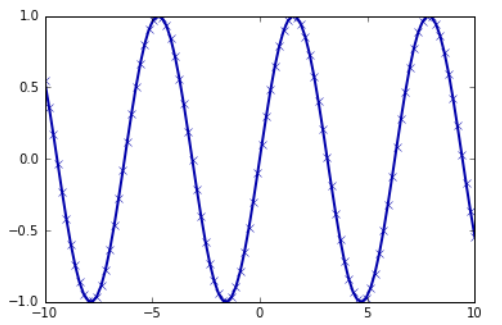
\includegraphics[scale=0.55]{Imagen_Machine/Seno}
	\caption{Gráfico de la función del seno usando matplotlib}
	\label{Seno}
\end{figure} 
                            %   wrangling   =   discusión  

\subsubsection{pandas}

 {\ttfamily pandas\index{pandas}} es basada en una estructura de datos llamada DataFrame, que es modelado como la DataFrame del software $R$. En términos sencillos, una DataFrame  panda  es una tabla, similar para una hoja de cálculo de Excel.  
   {\ttfamily pandas} provee un gran alcance de métodos para modificar e operar sobre esta tabla; en particular, permite  consultas con  SQL-like  y  asociacion  de tablas. En contraste con {\ttfamily NumPy}, que requiera que todas las entradas en el arreglo sean del mismo tipo,  {\ttfamily pandas} permite que cada columna sea un tipo separado (por ejemplo, enteros, fechas, números flotante, y cadenas de caracteres (strings) ). 
   Otra herramienta valiosa provista por pandas es su capacidad para tratar una gran variedad de formatos de archivo y bases de datos, como SQL, archivos de Excel, y archivos separado por comas (CSV).  Entrar  en detalle acerca de la funcionabilidad de {\ttfamily pandas} está fuera del alcance de este libro. Sin embargo, el texto \href{https://www.oreilly.com/library/view/python-for-data/9781449323592/}{\color{vino} Python for Data Analysis}  de  Wes McKinney (O’Reilly, 2012) provee una buena  guía.
   A continuación se presenta  un   ejemplo sencillo de una  DataFrame usando un diccionario:\\

\begin{lstlisting}	

In[7]:  import pandas as pd
        
        # create a simple dataset of people
        data = {'Name': ["John", "Anna", "Peter", "Linda"],
	            'Location' : ["New York", "Paris", "Berlin", "London"],
     	        'Age' : [24, 13, 53, 33]
               }
        
        data_pandas = pd.DataFrame(data)
        # IPython.display allows "pretty printing" of dataframes
        # in the Jupyter notebook
        #    display(data_pandas),   tambien muestra la tabla  display( )
        print(data_pandas) 
          
\end{lstlisting}  
    %     bonita =  pretty    

\noindent Este instrución  produce el siguiente resultado:
\begin{figure}[h!]
%	\centering
	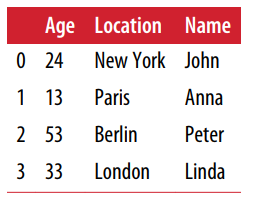
\includegraphics[scale=0.65]{Imagen_Machine/Captura}
%	\caption{Dataframe}
	\label{dataframe1}
\end{figure} 


Hay varias formas posibles de consultar esta tabla. Por ejemplo:\\

\begin{lstlisting}

In[8]:  # Select all rows that have an age column greater than 30
        display(data_pandas[data_pandas.Age > 30])

\end{lstlisting}

\noindent Esto produce el siguiente resultado:
\begin{figure}[h!]
	%\centering
	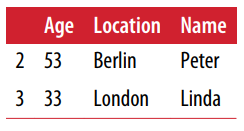
\includegraphics[scale=0.65]{Imagen_Machine/Dataframe2}
	%\caption{Dataframe}
	\label{dataframe2}
\end{figure} 



\subsubsection{mglearn}
 mglearn:\index{mglearn} Funciones  de ayuda para el libro "{}Introducción al aprendizaje automático con Python"{}.   Este libro viene con un código adjunto, que puede encontrar en \href{https://github.com/amueller/introduction_to_ml_with_python}{\color{vino} GitHub}.  El código adjunto incluye no sólo todos los ejemplos que se muestran en este libro, sino también
la librería {\ttfamily mglearn\index{mglearn}}.
  Ésta es una librería de utilidad funcional  que se emplea en este libro, así 
 que no saturamos listas de códigos con detalles para graficar  y carga los datos. Si
 está interesado, puede ver todas las funciones en el repositorio, pero los detalles del módulo  {\ttfamily mglearn}  no es realmente importante para el desarrollado del material de este libro.  Si hace un llamado a {\ttfamily mglearn} con el código, generalmente es una forma de hacer un trabajo rápido  y elegante, o para obtener  algunos datos interesantes.\\
        %     Throughout  =    A través   

  
\begin{minipage}[t]{0.2\textwidth}
	\centering\raisebox{\dimexpr \topskip-\height}{%
		
\includegraphics[width=\textwidth]{Imagen_Machine/Pajaro.png}}
\end{minipage}%\hfill
\begin{minipage}[t]{0.75\textwidth} 
	{\scriptsize		
		A lo largo del libro hacemos un amplio uso de NumPy, pandas  y matplotlib. 
		Todo el código asumirá las siguientes importaciones:
				
		\vspace{0.3cm} {\ttfamily
			
			{ \color{blue} 	importar numpy como np
				
				importar matplotlib.pyplot como plt
				
				importar pandas como pd
				
				importar mglearn\\  }  } 		

\begin{singlespace}
	También asumimos que ejecutará el código en un cuaderno Jupyter en línea con  \%matplotlib  habilitado para mostrar gráficos. Si no utiliza el cuaderno o estos comandos en linea (mágia de \%matplotlib), 	tendrás que usar el comando  plt.show  para  mostrar realmente cualquiera  de las figuras.
\end{singlespace}
}
\end{minipage}
  
   
  
   
   
\subsection{Python 2 Versus Python 3}

Hay dos versiones principales de Python\index{Python 2 Vs Python 3} que se usan ampliamente en este momento: Python 2 (más preciso, 2.7) y Python 3 (con la última versión 3.5 ó 3.7.4   en el momento de escribir y traducir este texto). Esto a veces conduce a cierta confusión.  Python 2 ya no está activamente en desarrollo,  pero debido a que Python 3 contiene cambios importantes, el código de Python 2 generalmente no no corre en Python 3. Si es Usted nuevo en Python o está comenzando un nuevo proyecto desde cero, recomendamos usar la última versión de Python 3 sin cambios.   Si Usted tiene una base de código grande en la que confía que está escrita para Python 2, está excusado de actualizarlo por ahora. Sin embargo, debe intentar migrar a Python 3 tan pronto como sea posible.  Si usted no tiene que interactuar con software heredado,  definitivamente debería usar a la Python 3.  Todo el código en este libro está escrito de una manera que funciona para ambas versiones. Sin embargo, el la salida exacta puede diferir ligeramente bajo  Python 2.

\subsubsection{Versiones utilizadas en este libro}

%  Previamente mencionamos  en las librerías
Las versiones usadas en este texto son las siguientes:
\begin{lstlisting}
In[9]:  import sys
        print("Python version: {}".format(sys.version))

        import pandas as pd
        print("pandas version: {}".format(pd.__version__))

        import matplotlib
        print("matplotlib version: {}".format(matplotlib.__version__))

        import numpy as np
        print("NumPy version: {}".format(np.__version__))

        import scipy as sp
        print("SciPy version: {}".format(sp.__version__))

        import IPython
        print("IPython version: {}".format(IPython.__version__))

        import sklearn
        print("scikit-learn version: {}".format(sklearn.__version__)) 
 
Out[9]:
    Python version: 3.7.4 (default, Aug  9 2019, 18:22:51) [MSC v.1915 32 bit (Intel)]
    pandas version: 0.25.1
    matplotlib version: 3.1.1
    NumPy version: 1.16.5
    SciPy version: 1.3.1
    IPython version: 7.8.0
    scikit-learn version: 0.21.1
\end{lstlisting}                        %         match  = coincidir encuentro
Si bien no es importante hacer coincidir exactamente estas versiones, usted debería tener una versión de scikit-learn que sea tan reciente como la que usamos. Ahora que tenemos todo establecido o configurado,  podemos ejecutar nuestra primera aplicación de  Aprendizaje Automático.\\


\begin{minipage}[t]{0.2\textwidth}
	\centering\raisebox{\dimexpr \topskip-\height}{%
		
\includegraphics[width=\textwidth]{Imagen_Machine/Escorpion}}
\end{minipage}%\hfill
\begin{minipage}[t]{0.75\textwidth} 
	{\scriptsize 
En este libro se supone que usted tiene la versión 0.18,  0.21.1  o  la más reciente de scikitlearn. El módulo model\_selection se agregó en 0.18. Si usas una versión anterior de scikit-learn, necesitará
ajustar lo más importante de este módulo.}
\end{minipage}\\



\section{Primera Aplicación:\\	
	 Clasificación de la especie de flores Iris}

En esta sección, empezaremos con una aplicación muy simple de aprendizaje automático y crearemos el primer modelo. Durante el proceso, introduciremos algunos términos y conceptos básicos.\\

Supongamos un botánico que se interesa en  distinguir  algunas especies de las flores  Iris que encontró. El ha coleccionado algunas medidas asociadas con cada una de las flores iris: La longitud y anchura tanto de los de los pétalos como la de los sépalos, todo medido en los centímetros (ver figura \ref{Iris} ).



\begin{figure}[h!]
	\centering
	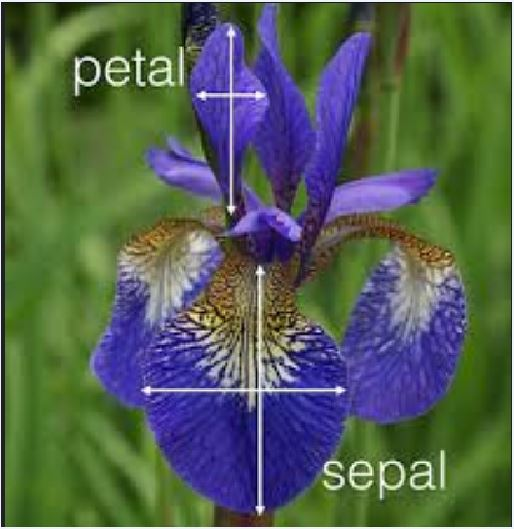
\includegraphics[scale=0.5]{Imagen_Machine/Iris}
	\caption{Partes de una flor especie Iris}
	\label{Iris}
\end{figure} 


Él también tiene las medidas de algunos flores iris que han sido previamente identificados por un botánico experto,  perteneciente a la especie  setosa, versicolor, y virginica (ver figura \ref{Especie}) Con esas medidas, él puede estar seguro a cuál especie pertenece cada iris. Supongamos que éstas son las únicas especie que nuestro botánico aficionado encontrará en su hábitat natural. 

Nuestro objetivo es construir un modelo de aprendizaje automático que pueda aprender de las mediciones
de estas flores iris cuya especie es conocida, para que podamos predecir la especie para una nueva flor
iris.\\


\begin{figure}[h!]
	\centering
	
\includegraphics[scale=0.5]{Imagen_Machine/Especie}
	\caption{Tres especies de flores Iris}
	\label{Especie}
\end{figure} 


Ya que tenemos las  medidas para las cuales conocemos la especie correcta de iris, éste es un problema de  de aprendizaje supervisado. En este problema, queremos predecir una  opciones de la especie de iris. Éste es un ejemplo de un problema de clasificación. Las posibles salidas (diferente especies de iris) son llamadas clases. 

Cada iris en el dataset pertenece a una de tres clases (setosa, versicolor, o virginica), este ejemplo es un problema de clasificación de tres clases. La salida deseada para un único punto de datos (una flor iris) es la especie de esta flor. Para un punto particular de la data, la especie a la que  pertenece es llamada  etiqueta, su etiqueta respectivamente.


\subsection{Data Iris}

Los datos que destinaremos para este ejemplo es la Dataset Iris, un conjunto de datos\index{dataset} (dataset) clásico en  las estadísticas y ahora en el aprendizaje automático. Está incluido en scikit-learn en el módulo de datasets. Lo podemos cargar llamando la función load\_iris:\\

\begin{lstlisting}
In[10]:  from sklearn.datasets import load_iris
         iris_dataset = load_iris()
\end{lstlisting}


El objeto  iris  que retorna al cargar  la data iris (load\_iris) es un objeto tipo manojo, lo cual es muy similar a un diccionario. Éste contiene claves y valores:\\

\begin{lstlisting}
In[11]:  print("Keys of iris_dataset: \n{}".format(iris_dataset.keys()))

Out[11]:  
    Keys of iris_dataset:
    dict_keys(['target_names', 'feature_names', 'DESCR', 'data', 'target'])
\end{lstlisting}

    %  feel free to look up the rest yourself

El valor de la  clave DESCR, es una descripción muy breve del conjunto de datos (dataset). Mostramos el inicio de la descripción aquí (usted puede ver el resto):\\

\begin{lstlisting}
In[12]:  print(iris_dataset['DESCR'][:193] + "\n...")

Out[12]:

    Iris Plants Database
    ====================
    Notes
    ----
    Data Set Characteristics:
       :Number of Instances: 150 (50 in each of three classes)
       :Number of Attributes: 4 numeric, predictive att
    ...
    ----
\end{lstlisting} 

El valor de la clave  {\ttfamily {target\_names}} es un arreglo  strings (matriz de cadena), conteniendo las especies de  las flores que queremos predecir:\\

\begin{lstlisting}
In[13]:  print("Nombre del objetivo: {}".format(iris_dataset['target_names']))

Out[13]:

Nombre del objetivo: ['setosa' 'versicolor' 'virginica']
\end{lstlisting}



El valor de {\ttfamily {feature\_names,}}  nombre de la característica es una lista de strings, que da la descripción de cada característica:\\

\begin{lstlisting}
In[14]:  print("Nombres de las Caracteristicas: \n{}".format(
                 iris_dataset['feature_names']))

Out[14]:

   Nombres de las Caracteristica:
   ['sepal length (cm)', 'sepal width (cm)', 'petal length (cm)',
    'petal width (cm)']
\end{lstlisting}

La data  contiene las medidas numéricas del ancho y longitud del sépalo y del pétalo,
  en un arreglo NumPy:\\


\begin{lstlisting}
In[15]:  print("Tipo de data: {}".format(type(iris_dataset['data'])))

Out[15]:

    Tipo de data: <class 'numpy.ndarray'>
\end{lstlisting}


Las filas en el arreglo de la data  corrresponden a las flores, mientras que las columnas representan las cuatro medidas que fueron tomadas a cada flor: 





\begin{lstlisting}
In[16]:  print("Forma de la data:  {}".format(iris_dataset['data'].shape))

Out[16]:
  
    Forma de la data:  (150, 4)
\end{lstlisting}



Vemos que el areglo (array) contiene las medidas de 150 flores diferentes. Recuerde
el item individual es llamado muestra en el aprendizaje automático, y sus propiedades son llamadas características. La forma del conjunto  de datos (array) es el número de muestras multiplicada por el número de características. Ésta es una convención en scikit-learn, y se asumirá que sus datos siempre están en esta forma. Aquí están los valores de característica para las primeras cinco muestras:\\

\begin{lstlisting}
In[17]:  print("Primeras 5 columnas de la data:\n{}".format(
                  iris_dataset['data'][:5]))

Out[17]:

   Primeras 5 columnas de la data:
   [[ 5.1  3.5  1.4  0.2]
    [ 4.9  3.   1.4  0.2]
    [ 4.7  3.2  1.3  0.2]
    [ 4.6  3.1  1.5  0.2]
    [ 5.   3.6  1.4  0.2]]
\end{lstlisting}



A partir de estos datos, podemos ver las primeras cinco flores tienen un ancho de pétalo de 0.2 cm
y que la primera flor tiene el sépalo más largo, de 5,1 cm. La matriz objetivo contiene las especies de cada una de las flores que se midieron, también como una matriz NumPy (NumPy array): \\

\begin{lstlisting}
In[18]:  print("Tipo de objetivo: {}".format(type(iris_dataset['target'])))

Out[18]:

    Tipo de objetivo: <class 'numpy.ndarray'>
\end{lstlisting}

  El objetivo es un arreglo unidimensional, con un entero por cada flor:\\ 

\begin{lstlisting}
In[19]:  print("Forma de objetivo: {}".format(iris_dataset['target'].shape))

Out[19]:

    Forma de objetivo: (150,)
\end{lstlisting}

  Las especies están codificadas con enteros del 0 al 2:\\

\begin{lstlisting}
In[20]:  print("Objetivo:\n{}".format(iris_dataset['target']))

Out[20]:
\end{lstlisting}
{ \ttfamily  	 {\scriptsize{ 
			
			Objetivo:
			
			[0 0 0 0 0 0 0 0 0 0 0 0 0 0 0 0 0 0 0 0 0 0 0 0 0 0 0 0 0 0 0 0 0 0 0 0 0
			
			\hspace{0.2cm}0 0 0 0 0 0 0 0 0 0 0 0 0 1 1 1 1 1 1 1 1 1 1 1 1 1 1 1 1 1 1 1 1 1 1 1 1
			
			\hspace{0.2cm}1 1 1 1 1 1 1 1 1 1 1 1 1 1 1 1 1 1 1 1 1 1 1 1 1 1 2 2 2 2 2 2 2 2 2 2 2
			
			\hspace{0.2cm}2 2 2 2 2 2 2 2 2 2 2 2 2 2 2 2 2 2 2 2 2 2 2 2 2 2 2 2 2 2 2 2 2 2 2 2 2
			
			\hspace{0.2cm}2 2] \\
			
}}}


El significado de los números estan dados por el arreglo   de la data iris 
 {\ttfamily iris['target\_names']}:  0 para Setosa, 1 para versicolor, y 2 para virginica.


%    trust   =  confianza
%    thumb    = general 

  %        performance  =  rendimiento 
  
\subsection{Mediendo el éxito: Datos para entrenamiento y prueba}

Queremos  construir un modelo con aprendizaje automático usando esta información que pueda predecir a la especie de iris para un nuevo conjunto de medidas. Pero antes de aplicar nuestro modelo a medidas nuevas, necesitamos conocer si realmente este modelo funciona bien, y si podemos confiar en sus predicciones. \\

% capital X,   lowercase y

Desafortunadamente, no podemos usar los datos que se emplean para construir el modelo para evaluarlo. Esto se debe a que el modelo siempre puede recordar simplemente todo el conjunto de entrenamiento, y por lo tanto siempre predecirá la etiqueta correcta para cualquier punto del conjunto de entrenamiento. Este
"{}recordatorio"{} no permite  indicar si el modelo se generalizará bien (en  otras palabras, si también funcionará bien con datos nuevos).


Para evaluar el rendimiento del modelo, lo tratamos o ejecutamos con nuevos datos (datos que no han visto
antes) para lo cual tenemos etiquetas. Esto generalmente se hace dividiendo los datos etiquetados que
hemos reunido (en este caso,  150 medidas de flores) en dos partes. Una parte de los datos se utilizan para construir el modelo de aprendizaje automático y se denominan datos de capacitación\index{conjunto de entrenamiento} o conjunto de entrenamiento. El resto de los datos se utilizarán para evaluar qué tan bien funciona el modelo; esta se llama datos de prueba, conjunto de prueba\index{conjunto de prueba} o conjunto de retención (test data, test set, or hold-out set).\\

scikit-learn contiene una función que baraja (seudoaleatorio) el conjunto de datos y lo divide: 
la función es {\ttfamily train\_test\_split}.  Esta función extrae el 75\% de las filas de los datos como
conjunto de entrenamiento, junto con las etiquetas correspondientes; y el 25\% restante
de los datos, junto con las etiquetas restantes, se declara como el conjunto de prueba. En este caso se ha decidido la cantidad de datos que desea dejar para el entrenamiento o capacitación  y  prueba del modelo,  con un criterio un poco arbitrario, sin embargo, usar un conjunto de prueba que contenga el 25\% de los datos es una buena regla general.   En scikit-learn, los datos generalmente se denotan con una $X$ mayúscula, mientras que las etiquetas se denotan por una $y$ minúscula. Esto está inspirado en la formulación estándar $f(x) = y$ en matemáticas, donde $x$ es la entrada de una función e $y$ es la salida. Siguiendo las convenciones de las matemáticas, usamos una $X$ mayúscula porque los datos son un arreglo bidimensional (un
matriz) y una $y$  minúscula  porque el objetivo es un arreglo unidimensional (un vector).


Apliquemos la instrucción {\ttfamily train\_test\_split} sobre nuestros datos y asignemos las salidas usando la siguiente  nomenclatura:\\

\begin{lstlisting}
In[21]:  from sklearn.model_selection import train_test_split
         X_train, X_test, y_train, y_test = train_test_split(
              iris_dataset['data'], iris_dataset['target'], random_state=0)

\end{lstlisting}


Antes de realizar la división, la función {\ttfamily train\_test\_split}  baraja el conjunto de datos utilizando un generador de números pseudoaleatorios. Si sólo tomamos los últimos 25\% de los datos como un conjunto de prueba, el conjunto de datos para la prueba  tendrían sólo la etiqueta 2, ya que los puntos de datos están ordenados por la etiqueta (observe la salida para  {\ttfamily iris['target']}  mostrada anteriormente). Usando un conjunto de prueba que sólo contenga una de las tres clases no nos dirá mucho sobre qué tan bien generaliza el modelo, entonces barajamos nuestros datos para asegurarnos de que los datos de prueba contengan datos de todas las clases.\\


Para asegurarnos  que obtendremos la misma salida si ejecutamos la misma función varias veces, proporcionamos al generador de números pseudoaleatorios una semilla fija usando el parámetro {\ttfamily random\_state}. Esto hará que el resultado sea determinístico, por lo que esta línea siempre tiene el mismo resultado. En este trabajo  fijaremos el {\ttfamily random\_state}, siempre que usemos un procedimiento aleatorio.\\



La salida de la función {\ttfamily train\_test\_split} \:es\: {\ttfamily X\_train, X\_test, y\_train}  y
{\ttfamily y\_test}, que son todos los arreglos {\ttfamily NumPy}.  {\ttfamily X\_train} contiene el 75\% de las filas del conjunto de datos,  y {\ttfamily X\_test} contiene el 25\% restante:\\

\begin{lstlisting}
In[22]:  print("X_train shape: {}".format(X_train.shape))
         print("y_train shape: {}".format(y_train.shape))

Out[22]:

    X_train shape: (112, 4)
    y_train shape: (112,)

In[23]:  print("X_test shape: {}".format(X_test.shape))
         print("y_test shape: {}".format(y_test.shape))

Out[23]:
    
    X_test shape: (38, 4)
    y_test shape: (38,)

\end{lstlisting}





      %   without = sin
\subsection{Primer paso: Analizar los datos}


Antes de construir un modelo de aprendizaje automático, es buena idea inspeccionar los datos,
para ver si la tarea se puede resolver fácilmente sin aprendizaje automático, o si la información deseada
podría no está contenida en los datos. Además, inspeccionar sus datos es una buena manera de encontrar anormalidades y peculiaridades.  Tal vez algunas de sus flores iris se midieron usando pulgadas y no centímetros, por ejemplo. En el mundo real, las inconsistencias en los datos y mediciones inesperadas son muy comunes.


Una de las mejores formas de inspeccionar los datos es visualizarlos. Una forma de hacerlo es mediante el uso de un gráfico de dispersión. Un diagrama de dispersión\index{gráfico de dispersión} de los datos coloca una característica a lo largo del eje $X$ y otra a lo largo del eje $Y$, y dibuja un punto para cada  datos (muestra). Lamentablemente, la pantalla de la computadora  tiene  sólo dos dimensiones,   lo que nos permite trazar sólo dos o tal vez tres características a la vez.  Es difícil trazar conjuntos de datos con más de tres características de esta manera. 

 
Una forma de tratar este problema es hacer un diagrama por pares, para analizar todos los pares posibles  de características. Si tiene una pequeña cantidad de características, como las cuatro que tenemos aquí, esta es bastante razonable. Sin embargo, debe tener en cuenta que un gráfico de pares no muestra la interacción de todas las funciones a la vez, por lo que algunos aspectos interesantes de los datos tal  vez no se revelarán al visualizarlo de esta manera.



La Figura \ref{pares} es un diagrama de pares dos a dos de las características en del conjunto de entrenamiento. Los puntos de datos están coloreados según la especie a la que pertenece la flor iris. Para crear  el gráfico, primero convertimos el arreglo {\ttfamily NumPy} en una { \ttfamily  Dataframe pandas. \:   pandas}  tiene una función para crear gráficos de pares llamado  {\ttfamily scatter\_matrix}. La diagonal de esta matriz se llena con los histogramas de cada característica:\\


\begin{lstlisting}
In[24]:  # create dataframe from data in X_train
         # label the columns using the strings in iris_dataset.feature_names
         iris_dataframe = pd.DataFrame(
                              X_train, columns=iris_dataset.feature_names)
         # create a scatter matrix from the dataframe, color by y_train
         grr = pd.scatter_matrix(iris_dataframe, c=y_train, figsize=(15, 15), 
                                 marker='o', hist_kwds={'bins': 20}, s=60, 
                                 alpha=.8, cmap=mglearn.cm3)
                             
\end{lstlisting}


\begin{figure}[h!]
	\centering
	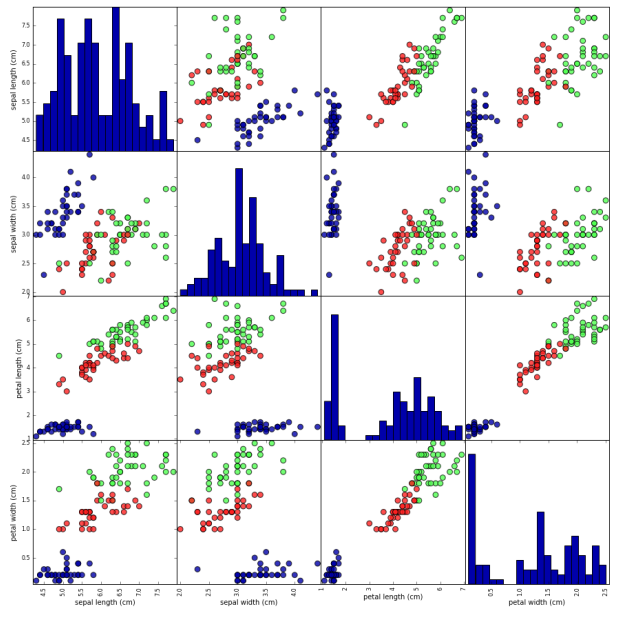
\includegraphics[scale=0.85]{Imagen_Machine/pares}
	\caption{Gráfico por pares de la dataset Iris, coloreado por etiquetas de clase}
	\label{pares}
\end{figure} 


De los gráficos en la figura \ref{pares}, podemos ver que las tres clases parecen estar relativamente bien separadas usando las medidas de sépalos y pétalos. Esto significa que un modelo de aprendizaje automático
probablemente podrá aprender a separarlos.



\subsection{Construyendo el Primer Modelo: método del k-Nearest Neighbors}

  %   k-vecinos más cercanos
Ahora podemos comenzar a construir el modelo real de aprendizaje automático. Hay muchos algoritmos de clasificación en {\ttfamily scikit-learn}  que podríamos usar. Aquí usaremos el clasificador del k-vecinos más cercanos (k-nearest neighbors\index{k-Nearest Neighbors}),  que es fácil de entender.   La construcción de este modelo sólo consiste en almacenar el conjunto de entrenamiento. Para hacer una predicción de un nuevo punto de datos, el algoritmo encuentra el punto en el conjunto de entrenamiento más cercano al nuevo punto, y luego asigna la etiqueta de este punto de entrenamiento al nuevo punto de datos.

La $k$ en el  k-vecinos más cercanos significa que en lugar de usar sólo el vecino más cercano
para el nuevo punto de datos, podemos considerar cualquier número fijo $k$ de vecinos en el conjunto de entrenamiento (por ejemplo, los tres o cinco vecinos más cercanos). Entonces, podemos hacer una predicción
utilizando la clase mayoritaria entre estos vecinos. Entraremos en más detalles sobre
esto en el Capítulo \ref{Cap2}; por ahora, usaremos un sólo vecino.\\


Todos los modelos de aprendizaje automático en {\ttfamily scikit-learn} son implementados en sus propias clases, y es llamado   {\ttfamily Estimator} de clases.  El algoritmo de clasificación del k-vecino más cercano es implementado en la clase  {\ttfamily KNeighboursClassifier}  en el módulo de {\ttfamily neighbors}.  Antes de usar el modelo, necesitamos instanciar la clase en un objeto\index{instanciar la clase}. Esto es cuando configuramos cualquier parámetro del modelo. 

El parámetro más importante  del  {\ttfamily KNeighboursClassifier}  es el número de vecinos, que estableceremos en 1:\\

\begin{lstlisting}
In[25]:  from sklearn.neighbors import KNeighborsClassifier
         knn = KNeighborsClassifier(n_neighbors=1)

\end{lstlisting}


  %    hold   =  sostiene  aguanta  guarda

El objeto knn encapsula el algoritmo que se usará para construir el modelo a partir de
la data de entrenamiento, así como el algoritmo para hacer predicciones sobre nuevos puntos de datos. Este
también contienen la información que el algoritmo ha extraído de los datos de entrenamiento.
 
En el caso de {\ttfamily KNeighboursClassifier}, sólo almacenará el conjunto de entrenamiento.
Para construir el modelo en el conjunto de entrenamiento, llamamos al método de ajuste del objeto knn,
que toma como argumentos el arreglo {\ttfamily NumPy \: X\_train} que contiene los datos de entrenamiento y
el arreglo NumPy y\_train de las etiquetas de entrenamiento correspondientes: \\

\begin{lstlisting}
In[26]:  knn.fit(X_train, y_train)

Out[26]:

    KNeighborsClassifier(algorithm='auto', leaf_size=30, metric='minkowski',
               metric_params=None, n_jobs=1, n_neighbors=1, p=2,
               weights='uniform')
\end{lstlisting}
    %        worry   =   preocupación 


El método de ajuste devuelve el objeto knn en sí (y lo modifica en su lugar), por lo que obtenemos una representación string\index{cadena de caracteres} (cadena de caracteres) de nuestro clasificador. La representación nos muestra qué parámetros fueron utilizados en la creación del modelo. Casi todos son valores predeterminados, pero puede también encontrar {\ttfamily n\_neighbours = 1}, que es el parámetro que seleccionamos. La mayoría de los modelos en scikit-learn tiene muchos parámetros, pero la mayor parte de ellos ya son  optimizaciones de velocidad o para casos de uso muy especiales. No tienes que preocuparte por los demás parámetros mostrados en esta representación.   Imprimir un modelo scikit-learn puede producir string  muy largas, pero no te dejes intimidar por estas. Cubriremos todo lo importante referente a parámetros en el Capítulo \ref{Cap2}. En el resto de este libro, no mostraremos el resultado  de ajuste porque no contiene ninguna información nueva.\\
         %  wild  = descabellado

\subsection{Haciendo Predicciones}

Ahora podemos hacer predicciones usando este modelo en nuevos datos para los cuales podríamos no conocer las etiquetas correctas. Imagina que encontramos un iris en la naturaleza con una longitud de sépalo de 5 cm, con  ancho de sépalo igual a 2,9 cm, una longitud de pétalo de 1 cm y un ancho de pétalo de 0,2 cm. ¿Qué especie de iris sería esta? Podemos poner estos datos en un arreglo  NumPy,  nuevamente  calcular la forma, es decir, el número de muestras (1) multiplicado por el número de características (4):\\

\begin{lstlisting}
In[27]:  X_new = np.array([[5, 2.9, 1, 0.2]])
         print("X_new.shape: {}".format(X_new.shape))

Out[27]:

    X_new.shape: (1, 4)
\end{lstlisting}



Observe  que realizamos las mediciones de esta flor individual en una fila en un arreglo NumPy bidimensional, ya que {\ttfamily scikit-learn}  siempre espera arrreglos bidimensionales para los datos.
Para hacer una predicción, llamamos el método de predicción del objeto knn:\\

\begin{lstlisting}
In[28]:  prediction = knn.predict(X_new)
         print("Predicion: {}".format(prediction))
         print("Nombre del objetivo estimado: {}".format(
                iris_dataset['target_names'][prediction]))

Out[28]:

    Predicion: [0]
    Nombre del objetivo estimado: ['setosa']
\end{lstlisting}


El modelo predijo que esta nueva flor iris pertenece a la clase 0, lo que significa que su especie es setosa.  Pero, ¿cómo sabemos si podemos confiar en nuestro modelo?  No sabemos la especie correcta de esta muestra, ¡cuál es el objetivo para completar de construir el modelo!


\subsection{Evaluación del modelo}

Aquí es donde entra el conjunto de prueba que creamos anteriormente. Estos datos no se utilizaron para construimos el modelo, pero conocemos la especie correcta para cada iris en el conjunto de prueba (test set).

Por lo tanto, podemos hacer una predicción para cada iris en el conjunto de prueba y compararlo contra su etiqueta (la especie conocida).  Podemos medir qué tan bien funciona el modelo calculando la  exactitud (accuracy)\index{exactitud}, que es la fracción de flores para la que se predijo la especie correcta:\\

\begin{lstlisting}
In[29]:  y_pred = knn.predict(X_test)
         print("Test set predictions:\n {}".format(y_pred))

Out[29]:

Test set predictions:
[2 1 0 2 0 2 0 1 1 1 2 1 1 1 1 0 1 1 0 0 2 1 0 0 2 0 0 1 1 0 2 1 0 2 2 1 0 2]

In[30]:  print("Test set score: {:.2f}".format(np.mean(y_pred == y_test)))

Out[30]:

    Test set score: 0.97
\end{lstlisting}


También podemos  usar el método de puntuación\index{método de puntuación} (score\index{score})  del objeto {\ttfamily knn}, que calculará la exactitud en el conjunto de prueba:\\


\begin{lstlisting}
In[31]:  print("Puntuacion del conjunto de pruebas: {:.2f}".format(
                 knn.score(X_test, y_test)))

Out[31]:

    Puntuacion del conjunto de pruebas: 0.97
\end{lstlisting}


Para este modelo, la exactitud del conjunto de prueba (test set) es de aproximadamente 0.97, lo que significa que hicimos la  predicción correcta  para el 97\% de los datos en el conjunto de prueba. Bajo  suposición estadística, esto significa que podemos esperar que nuestro modelo sea correcto el 97\% de la veces para nuevas flores iris.  
 La aplicación para el botánico aficionado, este alto nivel de exactitud significa que nuestro  modelo puede ser lo suficientemente confiable como para usarlo. En capítulos posteriores discutiremos cómo puede mejorar el rendimiento y las advertencias que existen al ajustar un modelo.


  %    trustworthy  =   confiable
  %     caveats     =   advertencias 



\section{Resumen y perspectivas}

Resumiendo lo que aprendido en este capítulo. Comenzamos con una breve introducción
al aprendizaje automático y sus aplicaciones, luego discutimos las diferencias entre
aprendizaje supervisado y no supervisado, y se dió una visión general de las herramientas que veremos
en este libro. Luego, formulamos la tarea de predecir  mediante el uso de medidas físicas  a qué especie  pertenece una nueva flor iris.  Utilizamos un conjunto de datos de mediciones que fue anotado por un experto con la especie correcta para construimos el modelo, convirtiéndolo en una tarea de aprendizaje supervisado. Había tres posibles especies, setosa, versicolor o virginica, que hace de la tarea un problema de clasificación de tres clases. Las especies posibles se denominan clases en el problema de clasificación, y la especie de una flor iris se llama su etiqueta. \\


El conjunto de datos Iris consta de dos arreglos {\ttfamily NumPy}: uno  contiene los datos  $X$  que son
referido  en {\ttfamily scikit-learn}, y el otro contiene los resultados correctos o deseados, llamados $y$.
El arreglo $X$ es una matriz bidimensional de características, con una fila para cada punto de datos o muestra y una columna por caraterística (o variable). El arreglo $y$ es una matriz unidimensional, que  contiene una clase de etiqueta, un número entero que varía de 0 a 2, para cada una de las muestras.


Dividimos el dataset (conjunto de datos\index{dataset}) en dos conjuntos, un conjunto para entrenar y construir el modelo, y el segundo conjunto de prueba para evaluar el modelo, y verificar qué tan bien  generaliza con los nuevos dato (datos no usados).


Elegimos el algoritmo de clasificación del k-vecinos más cercanos,  que hace las predicciones 
para un nuevo punto de datos considerando sus vecinos más cercanos en el conjunto de entrenamiento.  Esto es  implementado en el clasificador {\ttfamily  KNeighboursClassifier}, que contiene tanto el algoritmo que 
construye el modelo como   el algoritmo que realiza hace la predicción.


Instanciamos la clase, configurando los parámetros. Luego construimos el modelo llamando el
método de ajuste, tratando los datos de entrenamiento ({\ttfamily X\_train}) y las salidas de entrenamiento ( {\ttfamily y\_train}) como parámetros. Evaluamos el modelo utilizando el método de puntuación (score method), que calcula la exactitud  del modelo.  Aplicamos el método de puntuación (score method) a los datos de pruebas y conjunto de etiquetas, y encontramos que el modelo es aproximadamente 97\% exacto, lo que significa que es correcto 97\%  de la veces en el conjunto de prueba (test set).\\

En conclusión, el procedimiento generó un modelo que nos brinda  confianza para aplicarlo a nuevos datos (en este caso a nuevas medidas de flores)  y obtener aproximadamente el 97\%  de resultados correctos.\\


A continuación se presenta el resumen del código necesario para entrenar y evaluar el procedimiento:\\


\begin{lstlisting}
In[32]:  X_train, X_test, y_train, y_test = train_test_split(
             iris_dataset['data'], iris_dataset['target'], random_state=0)
         
         knn = KNeighborsClassifier(n_neighbors=1)
         knn.fit(X_train, y_train)
         
         print("Test set score: {:.2f}".format(knn.score(X_test, y_test)))

Out[32]:

    Test set score: 0.97
\end{lstlisting}

   %        snippet  =    fragmento

 Este fragmento contiene el  código nucléo (código básico) para aplicar cualquier algoritmo de aprendizaje automático usando scikit-learn.  Los métodos de ajuste, predicción y puntuación son interfaces comunes de los modelos supervisados es {\ttfamily scikit-learn}, y con los conceptos introducidos en este capítulo,
 pueden aplicar estos modelos a muchas tareas de aprendizaje automático.  En el próximo el capítulo, profundizaremos sobre los diferentes tipos de modelos supervisados en  {\ttfamily scikit-learn} y cómo aplicarlos con éxito.

%\end{document}

\newpage



